\subsection{Partie GMRES}
L'algorithme GMRES est utilisé pour résoudre de grands systèmes linéaires creux.
%
La plupart des opérations sont des opérations de type BLAS1 (axpy, dot product...) et sont facilement parallélisables.
%
L'opération la plus coûteuse de l'algorithme du GMRES est le produit matrice vecteur, ou {\em SpMV}\footnote{Sparse Matrix Vector multiply}.
%
Cette opération peut être parallélisée avec du parallélisme de boucle, les lignes de la matrice peuvent être traitées indépendamment les unes des autres.


Donc en général, l'algorithme GMRES se parallélise très bien.
%
Mais nous ne pouvons pas l'utiliser tel quel, nos matrices ne sont pas assez bien conditionnées.
%
Il est nécessaire de préconditionner nos matrices pour obtenir de bonnes performances.
%
Par contre, la partie préconditionneur n'est pas toujours facilement parallélisable.
%
Par exemple, le préconditionneur ILU(k), que nous allons utiliser, est un algorithme dont le parallélisme dépend de la structure de la matrice.
%
Cette structure dépend du problème traité ainsi que de la numérotation des cellules (Fig.~\ref{fig:matrix_ordering}).
%
Dans le cas d'une numérotation naturelle, il y a peu de parallélisme à exploiter.
%
Ce chapitre sera consacré à exploiter un maximum de parallélisme de l'algorithme ILU(k) en gardant une numérotation naturelle.

%   (-_-)   %
\begin{figure}[!ht]
     \begin{center}
        \subfigure[Numérotation naturelle des cellules.]{%
          \label{fig:matrix_natural_reservoir}
          
\includegraphics[width=0.49\textwidth]{matrix_natural_reservoir}
        }%
        \subfigure[Matrice associé à une numérotation naturelle.]{%
          \label{fig:matrix_natural_ordering}
          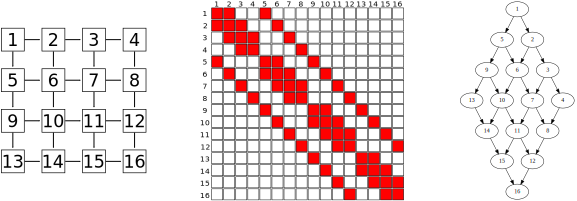
\includegraphics[width=0.49\textwidth]{matrix_natural_ordering}
        }\\%
        \subfigure[Numérotation rouge-noir des cellules.]{%
          \label{fig:matrix_redblack_reservoir}
          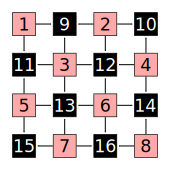
\includegraphics[width=0.49\textwidth]{matrix_redblack_reservoir}
        }%
        \subfigure[Matrice associé à une numérotation rouge-noir.]{%
          \label{fig:matrix_redblack_ordering}
          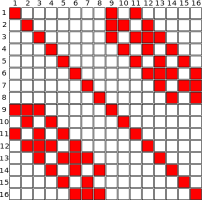
\includegraphics[width=0.49\textwidth]{matrix_redblack_ordering}
        }%
    \end{center}
    \caption{Impact de la numérotation sur la structure des matrices creuses.}
    \label{fig:matrix_ordering}
\end{figure}



%% \begin{algorithm}
%%   \fontsize{8pt}{9pt}\selectfont
%%     \begin{algorithmic}[1]
%%       \STATE Compute $r_0 := b - Ax_0$, $\beta := ||r_0||_2$, and $v_1 := r_0/\beta$
%%       \STATE Define the $(m + 1) x m$ matrix $\overset{-}{H}_m = \{h_{ij}\}_{1 \leq i \leq m+1, 1 \leq j \leq m}$. Set $\overset{-}{H}_m = 0$
%%       \FOR{$j=1$ to $m$}
%%         \STATE \tikz[baseline]{\node[fill=yellow!20,anchor=base]{Compute $temp := Triangular\_Solve(M, v_j)$};} \hspace{0.3in} (MPI\_Send(Border\_Cells))
%%         \STATE \tikz[baseline]{\node[fill=red!20,anchor=base]{Compute $w_j := A * temp$};} \hspace{1.2in} (MPI\_Recv(Ghost\_Cells))
%%         \FOR{\tikz[baseline]{\node[fill=blue!20,anchor=base]{$i=1$ to $j$};}}
%%           \STATE \tikz[baseline]{\node[fill=blue!20,anchor=base]{$h_{ij} := (w_j, v_i)$};}
%%           \STATE \tikz[baseline]{\node[fill=blue!20,anchor=base]{$w_j := w_j - h_{ij}v_i$};}
%%         \ENDFOR
%%         \STATE $h_{j+1,j} := ||w_j||_2$.
%%         \IF{$h_{j+1,j} = 0$}
%%           \STATE $m := j$
%%           \STATE \textbf{break}
%%         \ENDIF
%%         \STATE $v_{j+1} := w_j/h_{j+1,j}$
%%       \ENDFOR
%%       \STATE Compute $y_m$ the minimizer of $||\beta{}e_1 - \overset{-}{H}_my||_2$ and $x_m := x_0 + V_my_m$
%%     \end{algorithmic}
%%     \caption{GMRES with Householder orthogonalization from Yousef Saad}
%%   \end{algorithm}
